%% LyX 2.0.5.1 created this file.  For more info, see http://www.lyx.org/.
%% Do not edit unless you really know what you are doing.
\documentclass[usenatbib]{article}
\usepackage[latin9]{inputenc}
\usepackage[a4paper]{geometry}
\geometry{verbose}
\usepackage{color}
\usepackage{graphicx}

\makeatletter

%%%%%%%%%%%%%%%%%%%%%%%%%%%%%% LyX specific LaTeX commands.
%% A simple dot to overcome graphicx limitations
\newcommand{\lyxdot}{.}


%%%%%%%%%%%%%%%%%%%%%%%%%%%%%% Textclass specific LaTeX commands.
\usepackage{jcappub}

%%%%%%%%%%%%%%%%%%%%%%%%%%%%%% User specified LaTeX commands.






%%%%%%%%%%%%%%%%%%%%%%%%%%%%%% LyX specific LaTeX commands.
%% A simple dot to overcome graphicx limitations
%Make my life significantly easier
\usepackage{lineno}
\global\long\def\bd{{\bm{\delta}}}
 \linenumbers

\makeatother

\begin{document}

\title{Generating Mock Catalogs for the Baryon Oscillation Spectroscopic
Survey: An Approximate N-Body approach}


\author{Aaronson Aardvark...e.t.c.}


\abstract{We introduce and test an approximate scheme for generating mock catalogs
for large-scale structure measurements in galaxy surveys, specializing
in this work to the Baryon Oscillation Spectroscopic Survey. things
to add later...A brief description of the approximation scheme, tests
and the accuracy we reach, and some comments about the timings of
the tests and the BOSS sampes.}

\maketitle

\section{Introduction}

Why do we need large number of large N-body simuations? Discuss both
covariance matrix estimation as well as systematic error estimation.
Emphasize importance to capture as much of the physics as is possible...e.t.c.


\section{HACC}


\section{Convergence Test 1: Mass Resolution}

In this section, we investigate how mass resolution affects on halo
bias and mass functions. We prepare two samples with $256^{3}$ and
$512^{3}$ particles in the cubic box, whose side length is $256h^{-1}{\rm Mpc}$.
Note that both samples are simulated from the same initial density
field with the same number of time steps.

We first show comparison of cumulative mass functions in Figure \ref{fig:massFn_massResolution}.
We calculate mean and its error through the bootstrap method, generating
100 samples by choosing halos randomly from an output of the simulation.
In the right panel of Figure \ref{fig:massFn_massResolution}, the
mean and its error for the samples of $512^{3}$ particles are indicated
as shaded regions and the mean for $256^{3}$ particles indicated
as ci\textcolor{black}{rcles. The discrepancy in the mass functions
between $256^{3}$ particles and $512^{3}$ particles becomes larger
on large halo masses. This is mainly because there are a few large
halos and therefore it is more sensitive to the differences in the
number of halos. }\textcolor{red}{It is possible that samples with
higher mass resolutions resolve more small halos and a multiple halos
in the samples with $512^{3}$ particles correspond to one larger
halo in the $256^{3}$ particles samples.}\textcolor{black}{{} We also
see that agreement between the samples of those two mass resolutions
is better at lower redshift (}\textcolor{red}{How can I investigate
the reason for this?}\textcolor{black}{). }

In Figure \ref{fig:haloAuto_mass}, we compare halo-matter cross power
spectra at various redshifts. Here, we use the same matter density
field generated with $256^{3}$ particles for both cases, and we select
halos based on the ``soft-mass cut'' method using the probability
given by 

\begin{equation}
<N_{halo}(M)>=\frac{1}{2}{\rm erfc}(\frac{{\rm log(M_{cut}/}M)}{\sqrt{2}\sigma}),
\end{equation}
where we set ${\rm M_{cut}=10^{13.0}[{\rm M_{\odot}]}}$ and $\sigma=0.5$.
This probability has a similar form to the halo occupation distribution
(hereafter, HOD) technique so that the probability gradually becomes
one as increasing halo mass. We use this method to avoid noise from
halos scattering across sharp boundaries on halo mass. Using the soft
mass-cut method, we generate 10 samples to compute the cross power
spectra and their errors. From now on, we use the same method for
halo selections to compute power spectra. Note that the ratio of those
cross power spectra is equivalent to the ratio of halo bias. Figure
\ref{fig:haloAuto_mass} shows the halo bias for $256^{3}$ particles
is smaller than for $512^{3}$ particles and they agree well within
2\%. This also implies the effect on halo bias due to different mass
resolusion is less sensitive compared to the effect on mass functions. 

\begin{figure*}
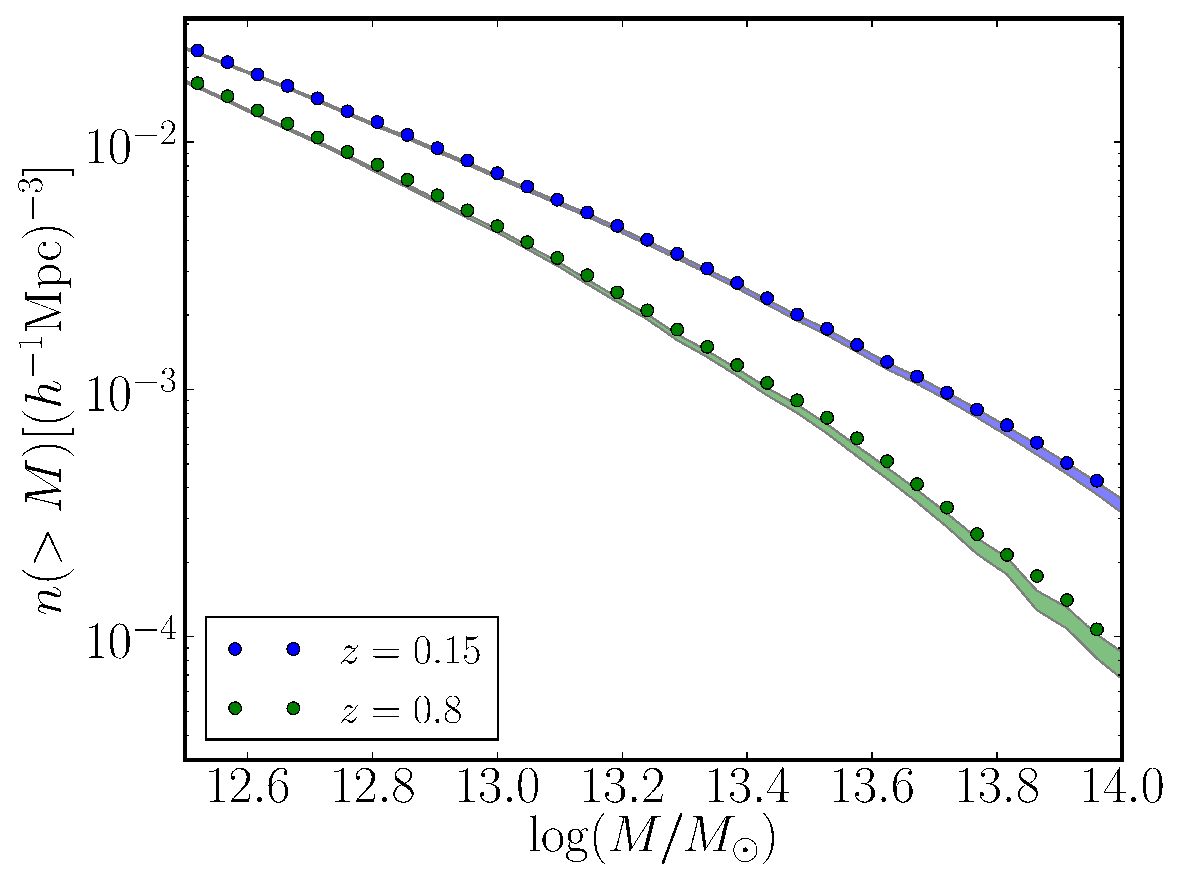
\includegraphics[width=0.5\columnwidth]{/Users/old_ts485/Dropbox/big-sims/Plots/haloNum_massResolution}\includegraphics[width=0.5\columnwidth]{/Users/old_ts485/Dropbox/big-sims/Plots/haloRatioNum_massResolution}

\caption{\label{fig:massFn_massResolution}Left: Cumulative mass functions
for the simulations of $512^{3}$ and $256^{3}$ particles. Shaded
regions are the mean with errors for the samples of $512^{3}$ particles
calculated through the bootstrap method. Circles are the mean for
$256^{3}$ particles. Right: Ratio of cumulative mass functions between
the samples of $512^{3}$ and $256^{3}$ particles. The deviation
from one on large halo masses is mainly caused by the fewer number
of large halos.}
\end{figure*}


\begin{figure}
\includegraphics[width=0.5\columnwidth]{/Users/old_ts485/Dropbox/big-sims/Plots/crossMatter_massRes_softMcut13\lyxdot 0_s0\lyxdot 5}

\caption{\label{fig:haloAuto_mass}Ratio of halo-matter cross power spectra
between the samples of $512^{3}$ and $256^{3}$ particles for various
redshifts. The overall agreements are all within 2\%. Note that halos
are selected based on the ``soft-mass cut'' method described in
the section.}
\end{figure}



\section{Convergence Test 2: Selection of the minimal time steps}

The goal in this section is to determine the sufficient time-stepping
scheme to resolve halo positions and masses reliably for the future
galaxy surveys. We are particularly interested in reducing the number
of sub\textcolor{black}{-cycles, because most of computational time
is spent in the short-range time solver. In order to quantitatively
evaluate different time-stepping schemes, we run a set of convergence
tests using smaller simulation boxes. We scale down these volumes
to $(256h^{-1}{\rm Mpc})^{3}$ with $256^{3}$ particles, which keeps
the particle mass unchanged. The number of time steps were chosen
as 450/5, 300/3, 300/2, 150/3, 150/2, where the first number indicates
the number of long time steps and the second number the number of
short time steps for each long time step. Note that all the samples
used in this section are at redshift $z=0.15$. After determining
our target time-stepping scheme, we do a more detailed examination
at various redshifts in the next section. To evaluate different choices,
we compare the properties (masses, positions, and velocities) of the
individual halos themselves in addition to the statistical descriptions
provided by the mass function and power spectra.}


\subsection{Matching }

Here, we compare halo properties by matching halos in different samples
one by one. We first show our algorithm for identifying the corresponding
halos in two different samples and then compare halo mass, position,
and velocity for those matched halos. From the quantitative comparison,
we find that the samples generated from the simulations with 300 global
steps have much less scatter for the baseline of the sample of the
450/5 simulation than the samples with 150 global steps. In addition
to that, we see that the differences between sub-cycles are almost
negligible.


\subsubsection{Algorithm}

Since our simulations all start with the same initial conditions,
we match halos in different simulations by matching their particle
content. Given a halo in simulation A, we consider the halos in simulation
B with the corresponding particles. Given this list of possible matches,
we match to the halo with the largest number of common particles.
To avoid spurious matches, we also require that the fraction of common
particles (relative to simulation A) exceeds a threshold. As an example
to illustlate how this matching algorithm works, we use the samples
from the 300/2 simulation and the 450/5 simulation. Figure \ref{fig:fraction1}
shows the cumulative fraction of unmatched halos matching the 450/5
simulation to the 300/2 simulation at $z=0.15$ with various thresholds.
As expected, the unmatched fraction increases with increasing threshold
and decreasing halo mass. We adopt a threshold of 50\% as our default
choice.

Since the above matching algorithm is unidirectional, multiple halos
in the sample A might be matched to a single halo in the sample B;
this happens 1 to 2\% of the time with a matching threshold of 50\%.
We refer to these as multiply-booked halos in what follows. Figure
\ref{fig:mass-scatter1} compares halo masses matching the 450/5 simulation
to the 300/2 simulation for the case of multiply-booked halos and
the rest. The top left panel shows a mass scatter for all the matched
halos between those two simulations, while the top right panel shows
a mass scatter only \textcolor{red}{for the non multiply-booked halos}.
The bottom panels show a mass scatter for the case of multiply-booked
halos. The bottom left panel shows a mass scatter for individual multiply-booked
halos, while we plots a summed halo mass for those corresponding halos
in the bottom right panel. As shown in the top left panel, there are
low-mass halos in the 450/5 simulation corresponding to high-mass
halos in the 300/2 simulation. The same trend is observed for the
case of multiply-booked halos, but not for the non multiply-booked
halos. Furthermore, those disagreement for halo masses between the
two simulations are resolved by adding the corresponding halo masses.
This implies that there are multiple halos in the 450/5 simulation
which are merged into one halo in the 300/2 simulation.

Figure \ref{fig:mass-content} shows the number densities of the unmatched
halos in the 450/5 simulation matching to the 300/2 simulation at
$z=0.15$. There are three reasons that halos are considered as unmatched.
First, if particles forming a halo in the sample A do not form a halo
in the sample B (i.e., halos in the samples do not share common particles),
we consider them as unmatched. Second, if the fraction of common particles
over the total number of particles in each halo is less than 50\%,
we eliminate halos for the case of spurious matching. At last for
the case of multiply-booked halos, we remove all but the one with
the largest number of common particles. We showed each unmatched number
density as a function of halo mass. We only find unmatched halos on
low-mass regions for the reason that the halos do not have any common
particles. This is because there are some low-mass halos which are
identified in one sample but not in another sample due to the way
the FOF algorithm define halos. As shown, most of unmatched halos
are due to the threshold criterion. \textcolor{black}{We also checked
how the number of matched halos is changed as a function of redshift,
and we observed that redshift does not affect to the matching algorithm.}

\begin{figure}
\includegraphics[width=0.5\columnwidth]{/Users/ts485/Dropbox/Tomomi/HACC/Conv/Matching_halos/particleID/unmatchedHalo_frac_450_300_2_z0\lyxdot 15}

\caption{\label{fig:fraction1}The cumulative fraction of unmatched halos matching
the 450/5 simulation to the 300/2 simulation at z=0.15 as a function
of halo mass. The solid lines, from top to bottom, correspond to matching
thresholds of 75\%, 50\%, and 25\% for the unmatched halos in the
450/5 sample. The dashed line shows the same quantity for the 300/2
sample for a threshold of 50\%. As expected, the unmatched fraction
increases with decreasing halo mass and increasing threshold. We adopt
a threshold of 50\% as our default choice. \textcolor{red}{Do we really
need the result for the 300/2 simulation?}}
\end{figure}


\begin{figure*}
\includegraphics[width=0.5\columnwidth]{/Users/old_ts485/Dropbox/Tomomi/HACC/Conv/Matching_halos/particleID/scatterMass_256_300_2_z0\lyxdot 15}
\includegraphics[width=0.5\columnwidth]{/Users/old_ts485/Dropbox/Tomomi/HACC/Conv/Matching_halos/particleID/testDB_nonDB_300_2_z0\lyxdot 15}

\includegraphics[width=0.5\columnwidth]{/Users/old_ts485/Dropbox/Tomomi/HACC/Conv/Matching_halos/particleID/testDB_DB_numPartCut_300_2_z0\lyxdot 15}
\includegraphics[width=0.5\columnwidth]{/Users/old_ts485/Dropbox/Tomomi/HACC/Conv/Matching_halos/particleID/testDB_sum_mass_f0\lyxdot 5_300_2_z0\lyxdot 15}

\caption{\label{fig:mass-scatter1}Comparison of halo masses matching the 450/5
simulation (x-axis) to the 300/2 simulation (y-axis) at $z=0.15$.
Panels correspond to halos with different matching criteria: all the
matched halos (top left), matched halos having one-to-one correspondence
(top right), matched halos not having one-to-one correspondence called
``multiply-booked'' halos (bottom left), and the ``multiply-booked''
halos whose corresponding halo masses are added (bottom right). Those
panels imply that large mass difference between the 450/5 simulation
and the 300/2 simulation shown in the top left panel is mainly because
those ``multiply-booked'' halos in the 450/5 simulation are merged
into one halo in the 300/2 simulation due to larger time steps.}
\end{figure*}


\begin{figure}
\includegraphics[width=0.5\columnwidth]{/Users/old_ts485/Dropbox/big-sims/Plots/unmatchHalo2_content_300_2_z0\lyxdot 15}

\caption{\label{fig:mass-content} Itemization of unmatched halos shown as
cumulative number densities of the unmatched halos from each procedure
in the matching algorithm. The solid line is the total and the dashed
lines correspond to matching based on particle content (green), elimination
due to the matching threshold (red), and elimination of ``multiply-booked''
halos (cyan). Most large halos being unmatched is due to the threshold. }
\end{figure}



\subsubsection{Halo Properties}

Here, we compare halo properties (i.e., halo mass, position, and velocity)
for halos matched to those in the 450/5 simulation. The comparison
of halo mass between the 450/5 simulation and the 300/2 simulation
at $z=0.15$ is shown in Figure \ref{fig:HaloProperty_mass}. Figure
\ref{fig:HaloProperty_mass} shows that the halos in the 300/2 simulation
tend to be slightly more massive than the corresponding halos in the
450/5 simulation. The panels in Figure \ref{fig:HaloProperty_step},
from left to right, show the comparison of halo position and velocity
for the matched halos at $z=0.15$. As shown, the 150 global steps
have more scatter in the halo properties and the means d\textcolor{black}{iffer
for the halo mass ratio }and the velocity difference. This indicates
that the halo structure in these cases is more diffused than the case
of the 300 or the 450 global steps. For the 300 global steps, the
results are significantly improved and the center position is matched
in these cases to better than 200 kpc. As is clear from Figure \ref{fig:HaloProperty_step},
the difference between 3 and 2 sub-cycles is negligible on halo properties.
Note that we observe the same trend in halo properties discussed here
at different redshifts.

\begin{figure*}[t]
\includegraphics[width=0.5\columnwidth]{/Users/old_ts485/Dropbox/Tomomi/HACC/Conv/Matching_halos/particleID/histogram_massDiff_z0\lyxdot 15}

\caption{\label{fig:HaloProperty_mass}Comparison of halo mass differencecs
for matched halos in the different simulations corresponding to the
time steps of 300/3 (blue), 300/2 (green), 150/3 (red), and 150/2
(cyan) with respect to the 450/5 simulation. \textcolor{red}{Talk
about this plot!!!}}
\end{figure*}


\begin{figure}
\includegraphics[width=0.5\columnwidth]{/Users/old_ts485/Dropbox/Tomomi/HACC/Conv/Test_correction/histogram_massSlice_z0\lyxdot 15}\includegraphics[width=0.5\columnwidth]{/Users/old_ts485/Dropbox/Tomomi/HACC/Conv/Test_correction/histogram_massSlice_z0\lyxdot 8}

\caption{XXX}


\end{figure}


\begin{figure*}[t]
\includegraphics[width=0.5\columnwidth]{/Users/ts485/Dropbox/Tomomi/HACC/Conv/Matching_halos/particleID/histogram_distance_z0\lyxdot 15}\includegraphics[width=0.5\columnwidth]{/Users/ts485/Dropbox/Tomomi/HACC/Conv/Matching_halos/particleID/histogram_velocity_z0\lyxdot 15}

\caption{\label{fig:HaloProperty_step}Comparison of matched halos in the different
simulations corresponding to the time steps of 300/3 (blue), 300/2
(green), 150/3 (red), and 150/2 (cyan) with respect to the 450/5 simulation.
From left to right, we compared halo position and velocity respectively.\textcolor{blue}{{}
}\textcolor{black}{The agreement between 300 global steps and the
450/5 simulation is considerably good, with little difference from
the number of sub-cycles.}}
\end{figure*}



\subsection{Observables}

We investigate how the number of time steps affects the observable
quantities including mass functions and power spectra.


\subsubsection{Time Steps}

We first compute mass functions from outputs of different time-stepping
schemes, as shown in Figure \ref{fig:massFn_step}, where we compare
simulations with reduced number of time steps to the 450/5 simulation.
In Figure \ref{fig:massFn_step}, we show the ratio $n(>M)/n_{450/5}(>M)$,
where $n_{450/5}(>M)$ is a cumulative mass function for the 450/5
simulation and $n(>M)$ is a cumulative mass function for different
time steps shown in different colors. We see that the cumulative mass
functions from the simulation with 150 global steps have smaller amplitudes
overall than those for the samples with 450 and 300 global steps.
This is because a smaller number of time steps makes halos more diffuse
and the fixed linking length cannot connect some particles in the
outputs of 150 global steps whose corresponding particles are connected
in the simulations of a larger number of global time steps. In \textcolor{red}{Manera
et al. 2012} which uses the second-order Lagrangian perturbation theory
to generate dark matter fields, they used a longer linking length
and reassigned halo masses in order to solve the same problem of having
diffused halos. We find that overall agreement between the 450/5 simulation
and the simulations with 300 global steps on mass functions is sufficient.

\begin{figure}
\includegraphics[width=0.5\columnwidth]{/Users/old_ts485/Dropbox/big-sims/Plots/haloRatioNum256_z0\lyxdot 15}

\caption{\label{fig:massFn_step} Comparison of cumulative mass functions in
different simulations taking the 450/5 simulation as a reference.
Lines, from top to bottom, correspond to the simulation with different
time steps, 300/3 (blue), 300/2 (green), 150/3 (red), and 150/2 (cyan)
respectively. As shown, the agreement between the simulations with
300 global steps and the 450/5 simulation is close to one on large
halo mass and sub-cycles make differences only on small halo mass.}
\end{figure}


The next measure of interest is the cross power spectra between halos
and matter densities, as shown in Figure \ref{fig:crossMater_step}.
Figure \ref{fig:crossMater_step} shows the ratio $P_{hm}/P_{hm,450/5}$
at $z=0.15$, where $P_{hm,450/5}$ is the cross power spectrum for
the 450/5 simulation and $P_{hm}$ is the cross power spectrum for
other time steps labeled in the figure. To calculate the cross power
spectra, we use the output of the 450/5 simulation for the matter
densities for all the halo samples. In this way, the ratio $P_{hm}/P_{hm,450/5}$
is equivalent to the ratio of halo bias between the 450/5 simulation
and the simulations with other time-steps. Note that the errors calculated
here are not due to sample variance, because we generate 10 samples
from one full sample by using the soft-mass cut method. We see that
the agreement between the 450/5 simulation and the simulations with
300 global steps is remarkably good and that the differences are well
within 2\% on any scales. In addition, we see the deviations on halo
biases for the simulations with 150 global steps are also within 5\%
from the halo bias for the 450/5 simulation on large scales. This
implies that halo bias on large scales is not largely affected by
reduction of the time steps.

\begin{figure}
\includegraphics[width=0.5\columnwidth]{/Users/old_ts485/Dropbox/Tomomi/HACC/Conv/Matching_halos/20130703/crossMatter_m450_timestep_softMcut13\lyxdot 0_s0\lyxdot 5_z0\lyxdot 15}

\caption{\label{fig:crossMater_step} Ratio of halo-matter cross pow\textcolor{black}{er
spectra as a function of time steps with respect to the 450/5. The
agreements with the 450/5 are all within 5\% on large scales. For
300 global steps, both agree well even on small scales with little
difference by sub-cycles. Note that the halos are selected based on
the soft mass-cut method with $M_{cut}=13.0$ and $\sigma=0.5$.}}
\end{figure}


As a conclusion through several convergence tests shown in this section,
we determine 300/2 as our optimal choice.


\section{Convergence Test 3: Tuning 300/2}

In the previous section, we choose the 300/2 simulation as our final
target for the time-stepping scheme. Now, we need to take a close
look at observable quantities calculated from the samples of the 300/2
simulation at various redshifts. Here, we first compare cumulative
mass functions between the 450/5 simulation and the 300/2 simulation
at redshifts $z=0.15$, $z=0.5$, and $z=0.8$ corresponding to different
colors shown in Figure \ref{fig:massFn_redshift}. As shown, an offset
from one increases with higher redshifts, particularly on small halo
masses. To make the mass functions for the 300/2 simulation closer
to the ones for the 450/5 simulation, we decided to reassign halo
masses for halos in the simulations of the 300/2 simulation.

\begin{figure}
\includegraphics[width=0.5\columnwidth]{/Users/old_ts485/Dropbox/big-sims/Plots/haloRatioNum_noTweak_redshift}

\caption{\label{fig:massFn_redshift}Comparison of cumulative mass functions
between the 450/5 simulation and the 300/2 simulation at $z=0.15$,
$z=0.5$, and $z=0.8$. For the larger redshifts, the deviation gets
larger particularly on small halo masses. }


\end{figure}



\subsection{method}

In order to compare halo mass differences between the 300/2 simulation
and the 450/5 simulation, we first match halos in the 300/2 simulation
to halos in the 450/5 simulation by using our matching algorithm.
Next, we take mean of the halo mass differences for those matched
halos as a function of halo mass of 300/2 and fit the mean to a functional
shown below,

\begin{equation}
M_{re}=M_{300/2}(1.0+\alpha(M_{300/2}/10^{12.0}[{\rm M_{\odot}])^{\beta},}
\end{equation}
where $M_{re}$ is a reassigned halo mass for the samples of 300/2,
$M_{300/2}$ is an original halo mass of 300/2, $\alpha$ and $\beta$
are free parameters which are functions of the redshift. By fitting
to the samples of the 300/2 simulation to the 450/5 simulation by
using the above functional, we find best fit parameters shown below:

\begin{equation}
\alpha(z)=0.123z+0.052,
\end{equation}
and
\begin{equation}
\beta(z)=-0.154z-0.447.
\end{equation}


Applying the functional to the samples from the 300/2 simulation,
we obtain mass functions shown in Figure \ref{fig:massFn_tweak}.
The match of reassigned halo mass functions for the 300/2 simulation
to the ones for the 450/5 simulation is significantly improved that
now the difference is well within 5\% on any halo masses at any redshifts.

\begin{figure}
\includegraphics[width=0.5\columnwidth]{/Users/old_ts485/Dropbox/big-sims/Plots/haloRatioNum_tweak5_redshift}

\caption{\label{fig:massFn_tweak}Comparison of cumulative mass functions after
reassigning halo masses for the 300/2 simulation. The agreement between
the 300/2 simulation and the 450/5 simulation is significantly improved
especially on halo masses greater than $10^{13.0}{\rm M_{\odot}}$.}
\end{figure}



\subsection{Power Spectra}

We calculate halo-matter cross power spectra after reassigning halo
masses for the 300/2 simulation, as shown in Figure \ref{fig:crossPower_redshift}.
We use halo mass thresholds of $10^{12.5}{\rm M_{\odot}}$ for the
left panel and $10^{13.0}{\rm M_{\odot}}$ for the right panel. As
expected from the mass functions, the match between the 300/2 simulation
and the 450/5 simulation with the threshold of $10^{13.0}{\rm M_{\odot}}$
is better than the one with $10^{12.5}{\rm M_{\odot}}$. The agreement
between the 300/2 simulation and the 450/5 simulation is, however,
well within 2\% for both cases, which is a significant improvement
compared to the results shown in the previous section.

\begin{figure}
\includegraphics[width=0.5\columnwidth]{/Users/old_ts485/Dropbox/Tomomi/HACC/Conv/Matching_halos/20130703/crossMatter_m450_tweak300_2_softMcut13\lyxdot 0_s0\lyxdot 5}

\caption{\label{fig:crossPower_redshift}Ratio of halo-matter cross power spectra
after reassigning halo masses for the sample from the 300/2 simulations.
We select halos based on the soft mass-cut method\textcolor{black}{{}
with $M_{cut}=13.0$ and $\sigma=0.5$. The overall agreements are
well within 2\%.}}


\end{figure}



\section{THE BOSS SIMULATIONS}


\subsection{Simulation Parameters}


\subsection{Building the Galaxy Catalog}


\subsection{An Application}
\end{document}
